\documentclass[debug]{beamer} % beamer 3.10: do NOT use option hyperref={pdfpagelabels=false}! 
%\documentclass[final,hyperref={pdfpagelabels=false}]{beamer} % beamer 3.07: get rid of beamer warnings


\renewcommand*\oldstylenums[1]{{\firaoldstyle #1}}

\mode<presentation>{\usetheme{dsunicamp}}


% Put any other packages or custom macros in here:
\PassOptionsToPackage{main=english}{babel}
\usepackage[english]{babel}
\usepackage[utf8]{inputenc}		% Codificacao do documento (convers\~{a}o autom\'{a}tica dos acentos)
\usepackage[T1]{fontenc}
\usepackage[backend=biber, isbn=false, doi=false,style=ieee,language=english]{biblatex}
\renewcommand*{\bibfont}{\footnotesize}
\setbeamercolor{bibliography item}{parent=palette primary}
\setbeamercolor*{bibliography entry title}{parent=palette primary}
\bibliography{bibliography}


%%%%%%%MATH STUFF
\usepackage{fix-cm}% just to avoid some spurious messages
\usepackage{amsmath}
\usepackage{mathtools}
\usepackage{bm}
\usepackage{exscale} %integral sign in poster
\usepackage{eulervm}
%%%%%%%%%RANDOM STUFF
\usepackage{cleveref} %cref, Cref
\usepackage{microtype} %aligning and stuff
%%%%%%%%%GRAPHICAL STUFF
\usepackage{tikz}
\usepackage{mdframed}
\usepackage{subcaption} %subfigs
\usepackage{graphicx}% http://ctan.org/pkg/graphicx
\usetikzlibrary{calc}

% Portrait, A0 poster. Set scale as desired, but 1.3 gives easily readable text when printed.
\usepackage[orientation=portrait, size=custom, scale=1.3,width=91.44,height=121.92]{beamerposter}
% Set height of page for use in arranging text boxes, after accounting for
% heading, footer etc. This is a bit of a hack, ideally latex should figure
% this out for itself!
% \usepackage{geometry}
% \geometry{paperwidth=3ft, paperheight=5ft}

\newlength{\columnheight}
%133cm is all that remains
\setlength{\columnheight}{100cm}

\pdfstringdefDisableCommands{%
  \def\\{ }%
  \def\vspace{0.3em}{ }%
}



\newcommand{\hcurl}[1]{H (curl;#1)}
\newcommand{\hzcurl}[1]{H_0(curl;#1)}
\newcommand{\hone}[1]{H^1(#1)}
\newcommand{\hmspace}[1]{H^m(#1)}
\newcommand{\hzone}[1]{H^1_0(#1)}
\newcommand{\testhcurl}[0]{\bm{\varphi}}
\newcommand{\testhone}[0]{\varphi}
\newcommand{\pkspace}[2][k]{\mathbb{P}_{#1}(#2)}
\newcommand{\pkhomospace}[2][k]{\sim{\mathbb{P}}_{#1}(#2)}
\DeclareMathOperator{\curlop}{\nabla \times}
\DeclareMathOperator{\divop}{\nabla \cdot}
\DeclareMathOperator{\gradop}{\nabla}
\DeclareMathOperator{\curlopt}{\nabla_t \times}
\DeclareMathOperator{\divopt}{\nabla_t \cdot}
\DeclareMathOperator{\gradopt}{\nabla_t}

% Define the header information
\title{DEVELOPMENT OF HIGH-ORDER\\ \vspace{0.3em} \texorpdfstring{H(CURL,$\Omega$)}{H(CURL,OMEGA)}-CONFORMING APPROXIMATION SPACES FOR PHOTONIC WAVEGUIDE ANALYSIS}
% \title{Title \\ \vspace{0.3em} second line of title}
\author{Francisco T. Orlandini\texorpdfstring{\textsuperscript{1}}{ }, Hugo E. H. Figueroa\texorpdfstring{\textsuperscript{1}}{ } and Philippe R. B. Devloo\texorpdfstring{\textsuperscript{2}}{ }}
\institute{\texorpdfstring{\textsuperscript{1}}{ }School of Electrical and Computer Engineering, University of Campinas, Campinas-SP 13083-852, Brazil\\
\texorpdfstring{\textsuperscript{2}}{ }School of Civil Engineering, Architecture and Urban Design, University of Campinas, Campinas-SP 13083-852, Brazil}%

% Now start the actual poster
\begin{document}

% Header is automatically generated from the command defined in the theme
% file, the information above and the logos in the logo folder.


% Start of the body:
\begin{frame}
  \begin{columns}

    %% Left column:
    %% ============================================================
    \begin{column}{0.45\textwidth}

      % For some reason we need parbox to get it to arrange the boxes
      % with evenly spaced gaps
      \parbox[t][\columnheight]{\textwidth}{

        \vfill % vfill between every block so that everything is
               % automatically nicely spaced out.

        \begin{block}{ABSTRACT}
          \begin{itshape}   % italic abstract
          	\begin{itemize}
          		\item Photonics is hard.
          		\item Real hard.
          		\item People say FEM is crap and pseudospectral methods are the only option.
          		\item This is actually not true and I will show you why.
          	\end{itemize}
             % The advances in the fabrication of photonic waveguides in the past twenty years have led the scientific community to seek for numerical methods that could assist in the process of design of such devices. The design photonic waveguides often require relative errors of $10^{-14}$ on the dispersion parameters. In this context, a hierarchical strategy for constructing $\hcurl{\Omega}$-conforming elements is introduced, for application in a Finite Element Method (FEM) scheme for modal analysis of electromagnetic waveguides. The hierarchical $\hcurl{\Omega}$-conforming elements are used for the transversal component of the electric field, coupled with scalar $\hone{\Omega}$ elements for its longitudinal component. The Nédélec elements of the first kind were chosen for this work, and the ease of integration with \emph{p}-adaptivity schemes motivated the hierarchical construction of the FE basis. The scheme is assessed by means of the analysis of well-known waveguides. As a real-world scenario, the modal analysis of a Photonic Crystal Fiber illustrates the accuracy and the generalized eigenvalue problem size when dealing with a design process requiring high precision on the dispersion parameters.
            \end{itshape}
        \end{block}

        \vfill
        \begin{block}{\boxnumber FEM FORMULATION AND THE \texorpdfstring{H(CURL,$\Omega$)}{H(CURL,OMEGA)}-CONFORMING ELEMENTS}
        The formulation used in this work perform modal analysis on the cross-section of a waveguide, $\Omega$, for a given frequency and it uses $\hcurl{\Omega}$ and $\hone{\Omega}$-conforming elements for the transverse and longitudinal components of the electric field, respectively. It is valid for a domain composed of materials presenting at most transverse-anisotropy. From \textcite{jin14}:

	        Find non-trivial $\left(\beta^2,{e_t}, {e_z}\right) \in (\mathbb{C} \times [\mathbb{C}]^N \times [\mathbb{C}]^M)$ such that:
			\begin{equation}
				\renewcommand{\arraystretch}{1.5}%
	  			 \scalebox{0.9}{% Scale
					$\begin{multlined}\label{eq:fem-hcurl-disc-1}
					    \int_\Omega\left\{\sum_{j}^Ne_{tj}\left[\mu_{zz}^{-1} \left( \nabla_t \times \testhcurl_j \right)\cdot \left( \nabla_t \times \testhcurl_i \right)^*- k_0^2 \bm{\epsilon}_{xy}\testhcurl_j\cdot\testhcurl_i^*\right]\right.\\
					     +\left.\beta^2\sum_{l}^M e_{zk} \left[ \sum_{j}^Ne_{tj} \bm{\mu}_{xy^S}^{-1} \left( \nabla_t \testhone_k +\testhcurl_j \right)\cdot \left(\nabla_t \testhone_k +\testhcurl_i \right)^*-k_0^2\epsilon_{zz} \testhone_k\testhone_k^*\right]\right\}\mathrm{d}\Omega = 0,\\
					     \forall \testhcurl_i \in B_{U_h}\,,\, \testhone_k \in B_{V_h}\text{,}
					\end{multlined}$
				}
			\end{equation}%
			where $B_{U_h}$ and $B_{V_h}$ denote the FEM basis for the finite-dimensional subspaces of $\hcurl{\Omega}$ and $\hone{\Omega}$, respectively.

			The  $\hcurl{\Omega}$-conforming elements are the Nédélec elements of the first kind \textcite{nedelec80} and were constructed in the NeoPZ framework in a hierarchical way.
        \end{block}

        \vfill
        \begin{block}{\boxnumber EFFECTS OF GEOMETRICAL REPRESENTATION}
        	When you use high order elements you must be careful with the geometry. Otherwise your results will be crap. Check this out.

        	\begin{figure}[ht]
	            \centering
	            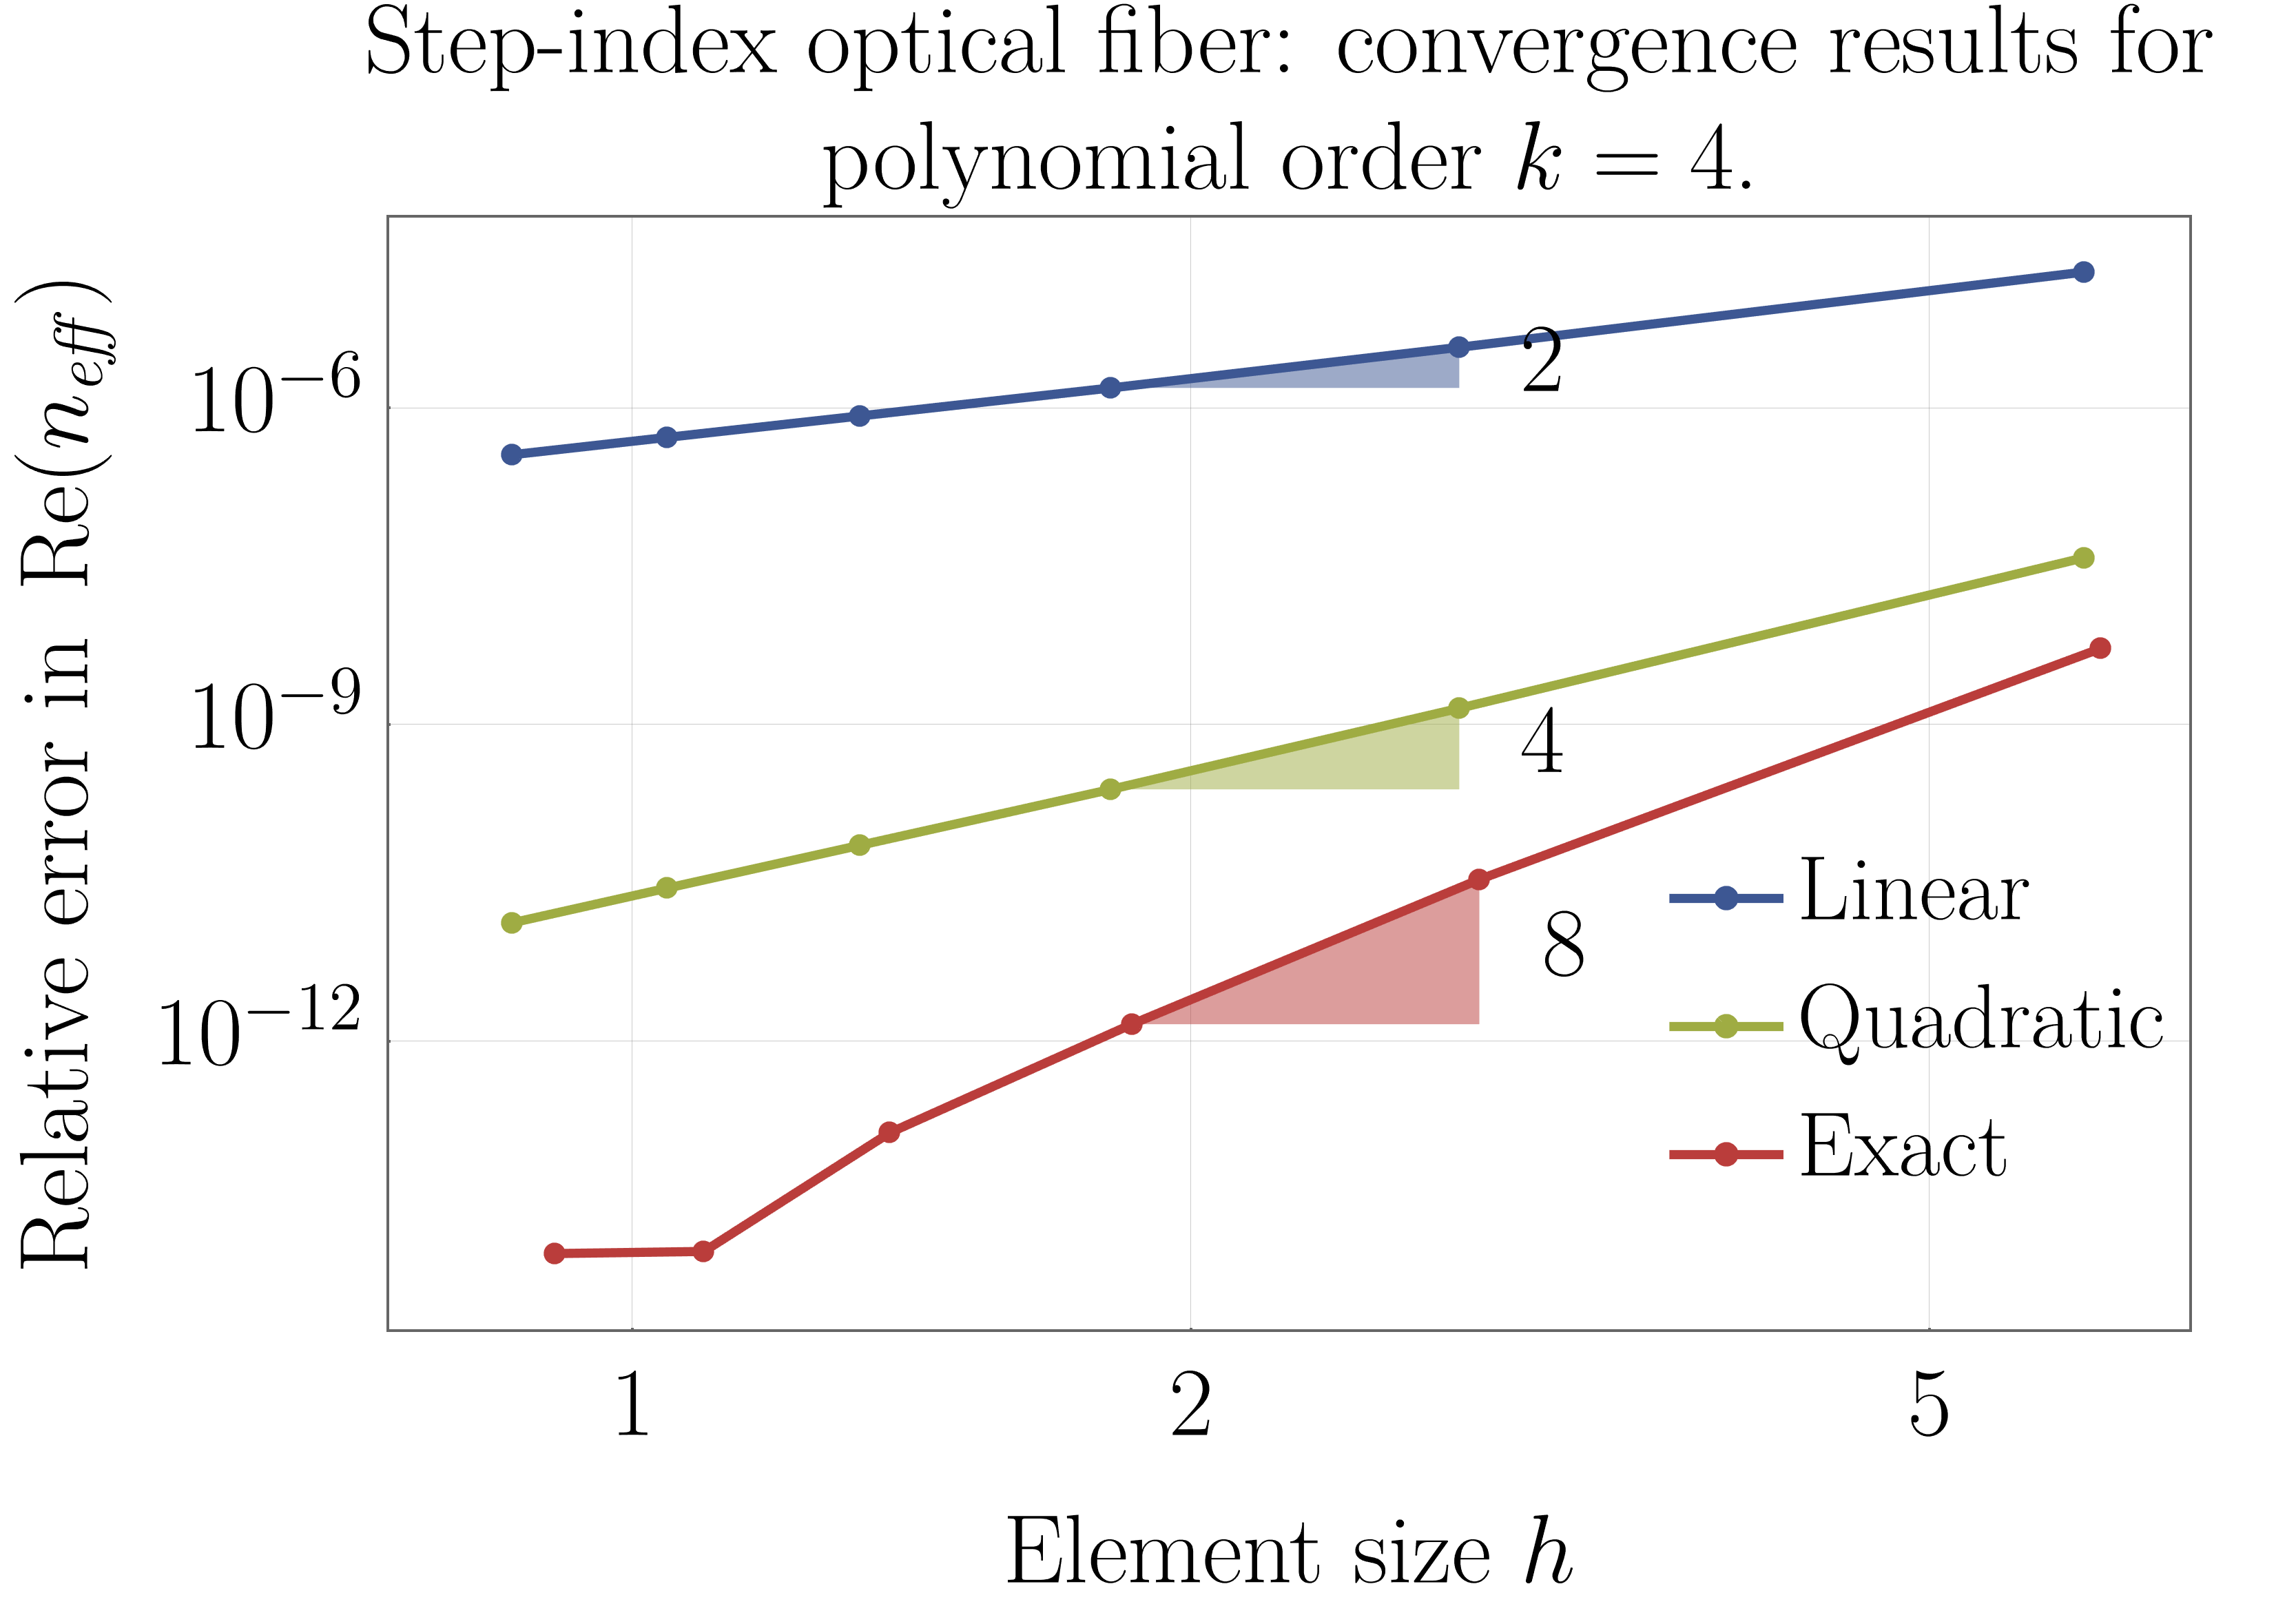
\includegraphics[width=0.7\linewidth]{images/convergenceRates_k4_poster.png}
	            \caption{Comparison of convergence rates for the real part of the effective index of a step-index optical fiber. The polynomial order $k=4$ was used in all three approximations. The geometry was described with elements obtained by linear mapping(blue curve), quadratic mapping(green curve) and exact mapping(red curve).}
	            \label{fig:convergence-step}
        	\end{figure}
        
	        Etc

	        \begin{figure}[hb]
	        	\begin{mdframed}[backgroundcolor=bggrey]
					\centering
					\begin{subfigure}[b]{.4\textwidth}
						\centering
						\caption*{$\displaystyle\bm{E}_t$}
						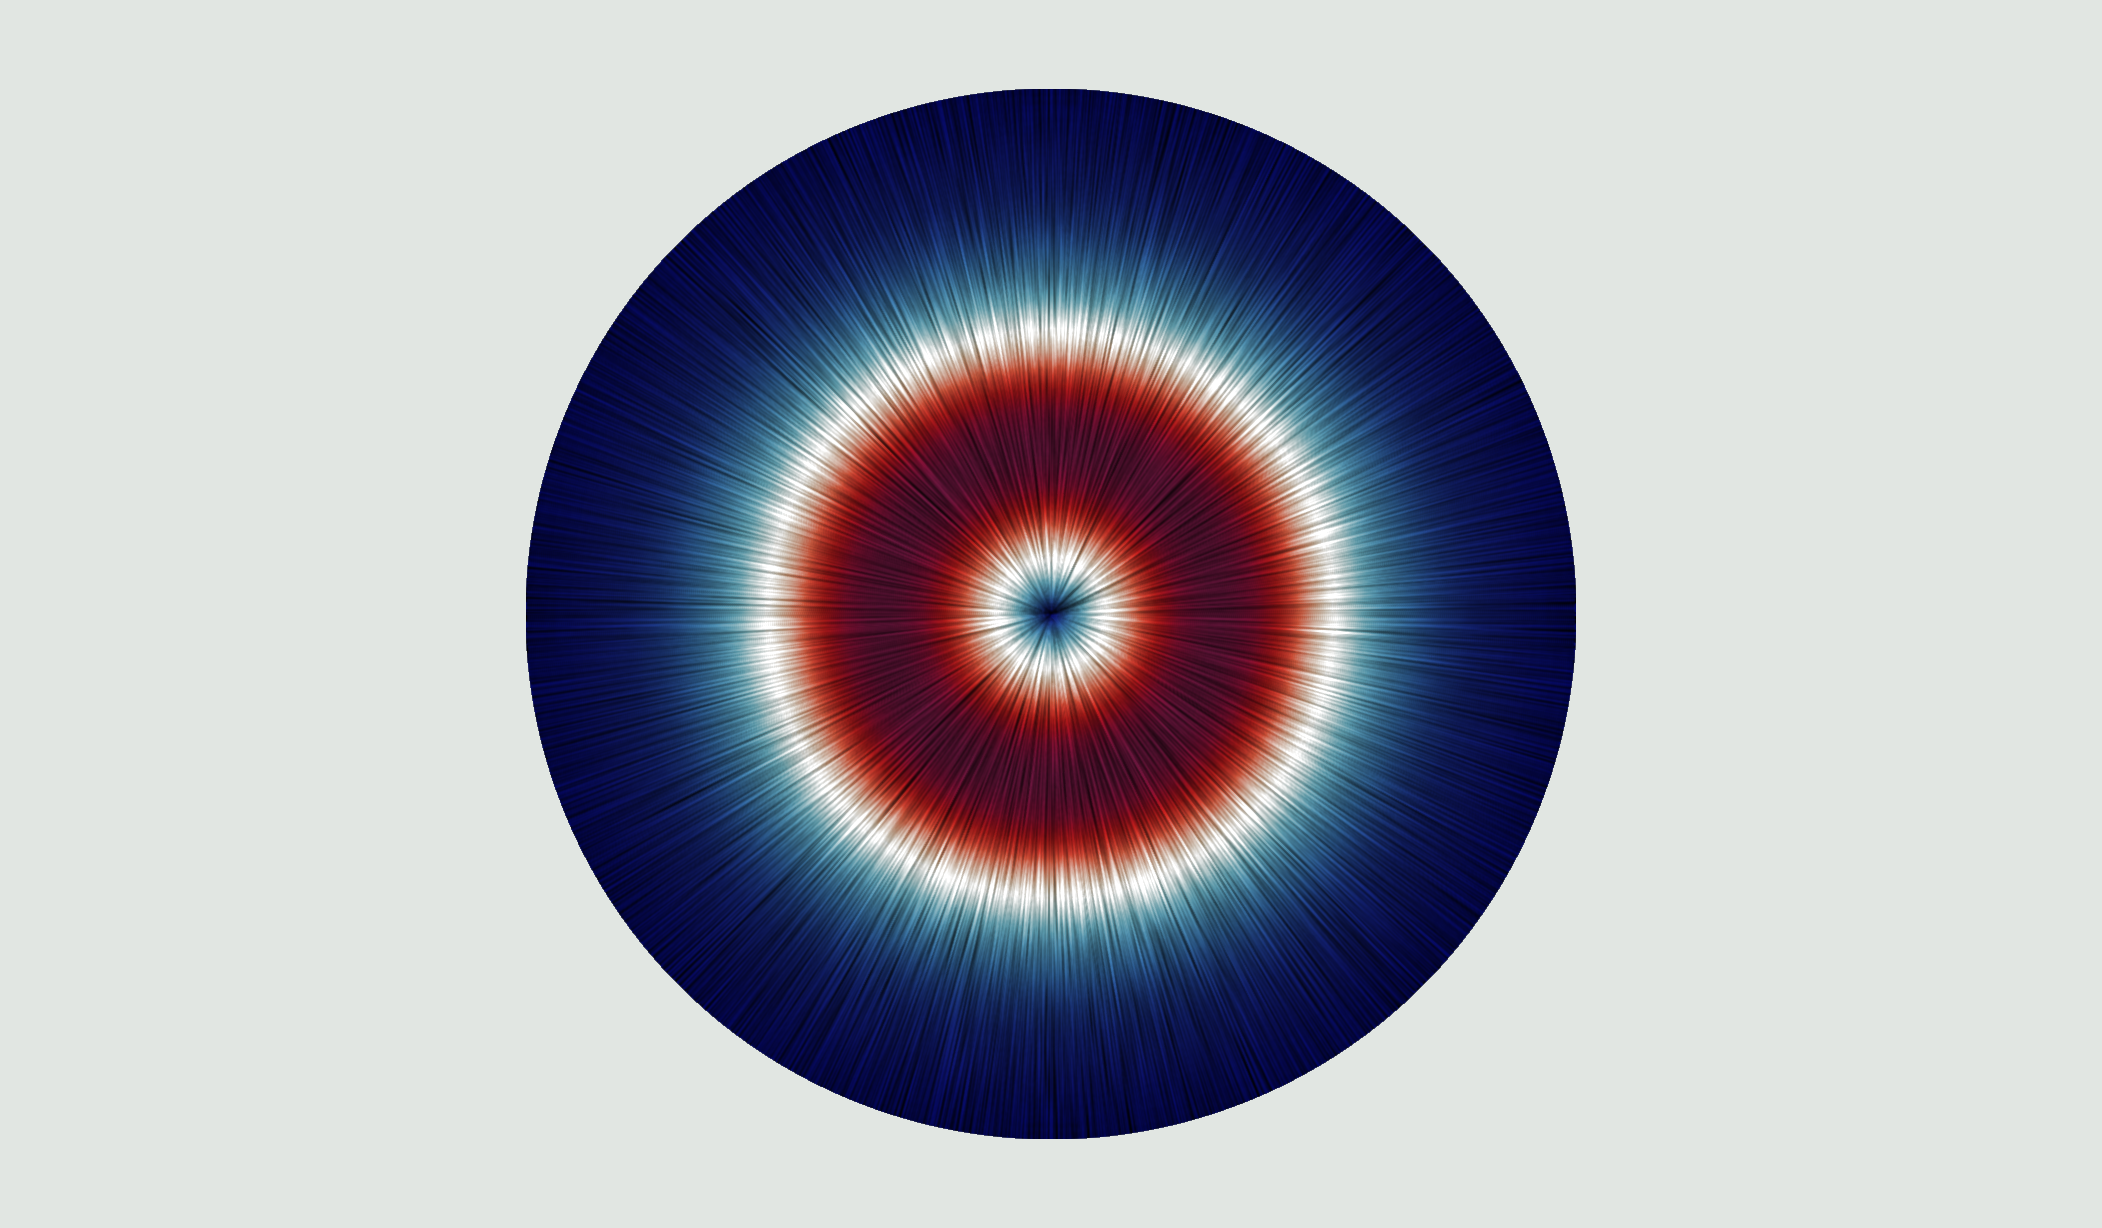
\includegraphics[width=1\linewidth]{images/et2posterStepFiber.png}%
					\end{subfigure}\hfill
					\begin{subfigure}[b]{.4\textwidth}
						\centering
						\caption*{$\displaystyle E_z$}
						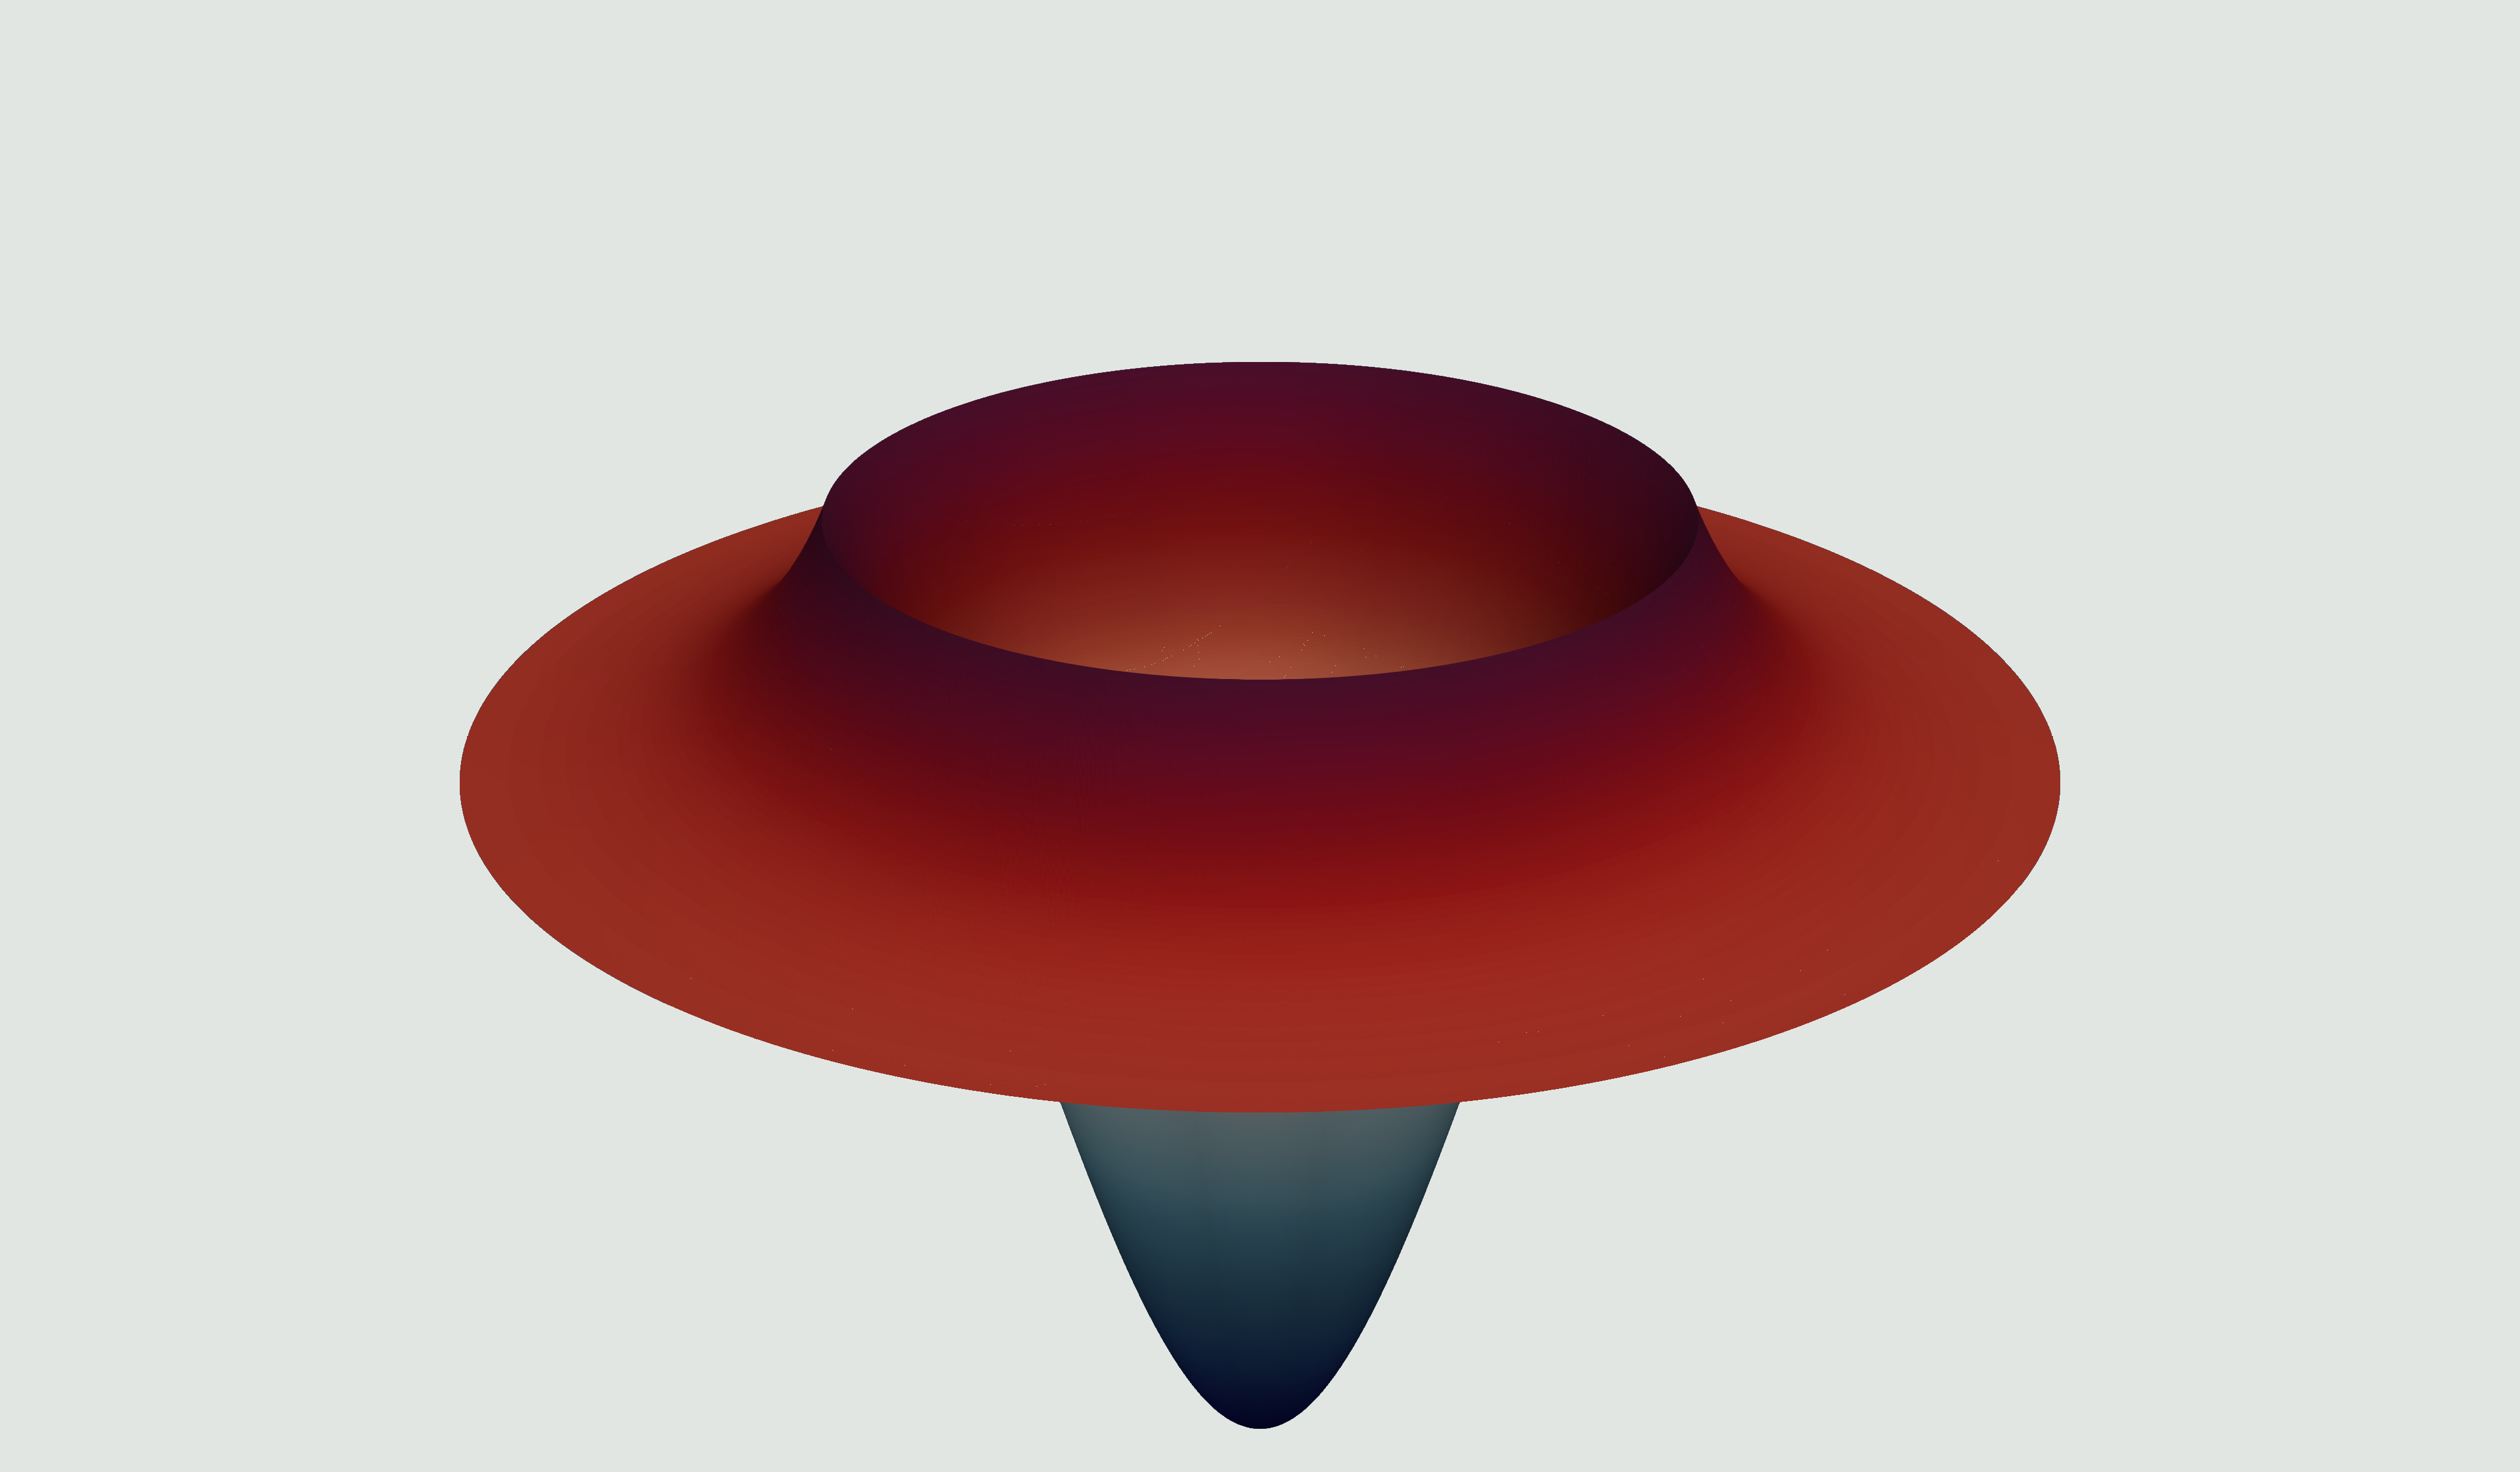
\includegraphics[width=1\linewidth]{images/ez2posterStepFiber.png}%
					\end{subfigure}

					\begin{subfigure}[b]{.4\textwidth}
						\centering
						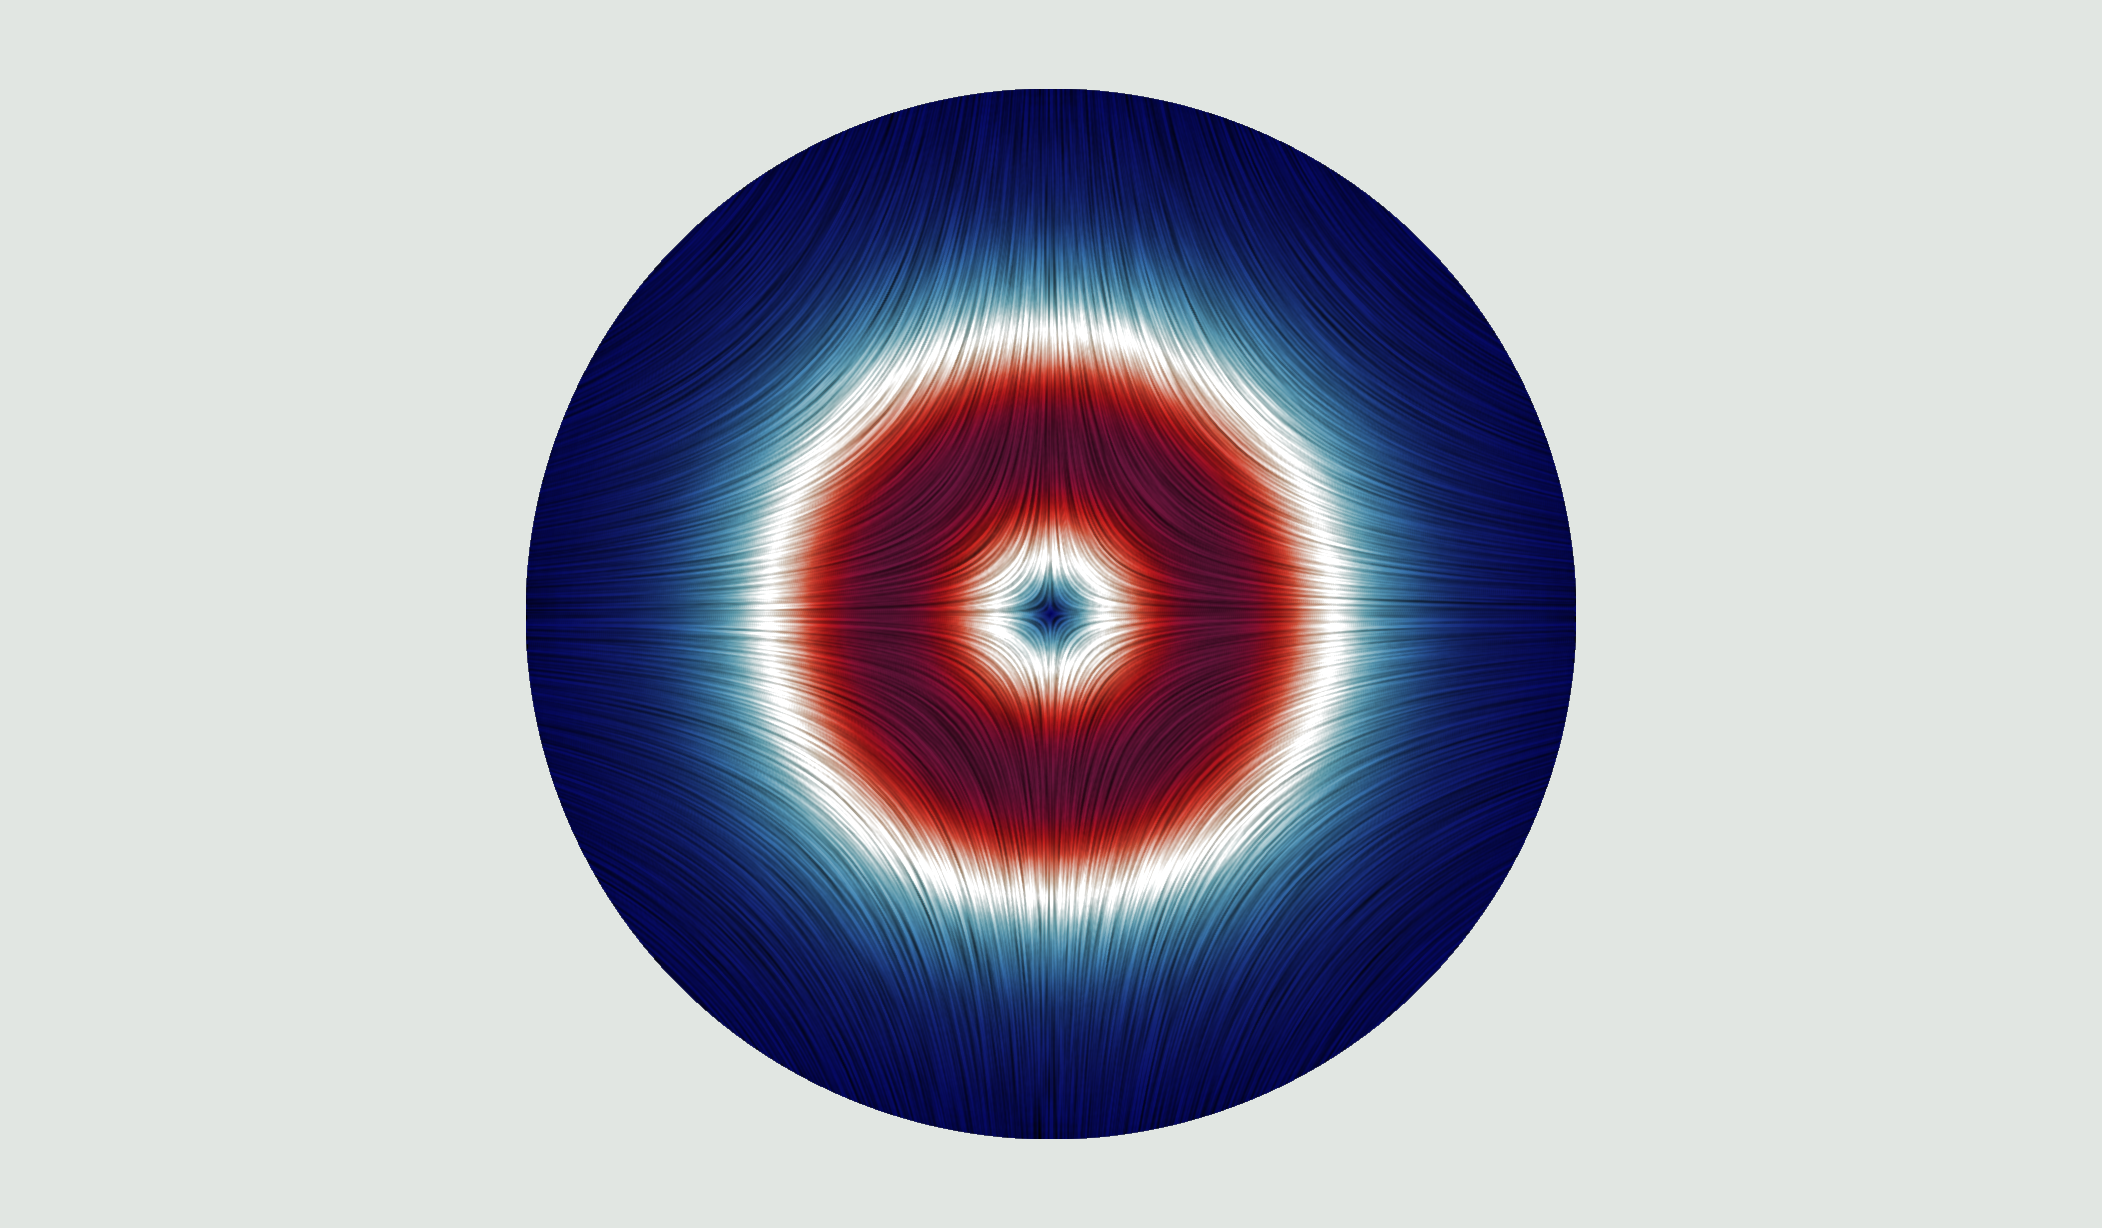
\includegraphics[width=1\linewidth]{images/et3posterStepFiber.png}%
					\end{subfigure}\hfill
					\begin{subfigure}[b]{.4\textwidth}
						\centering
						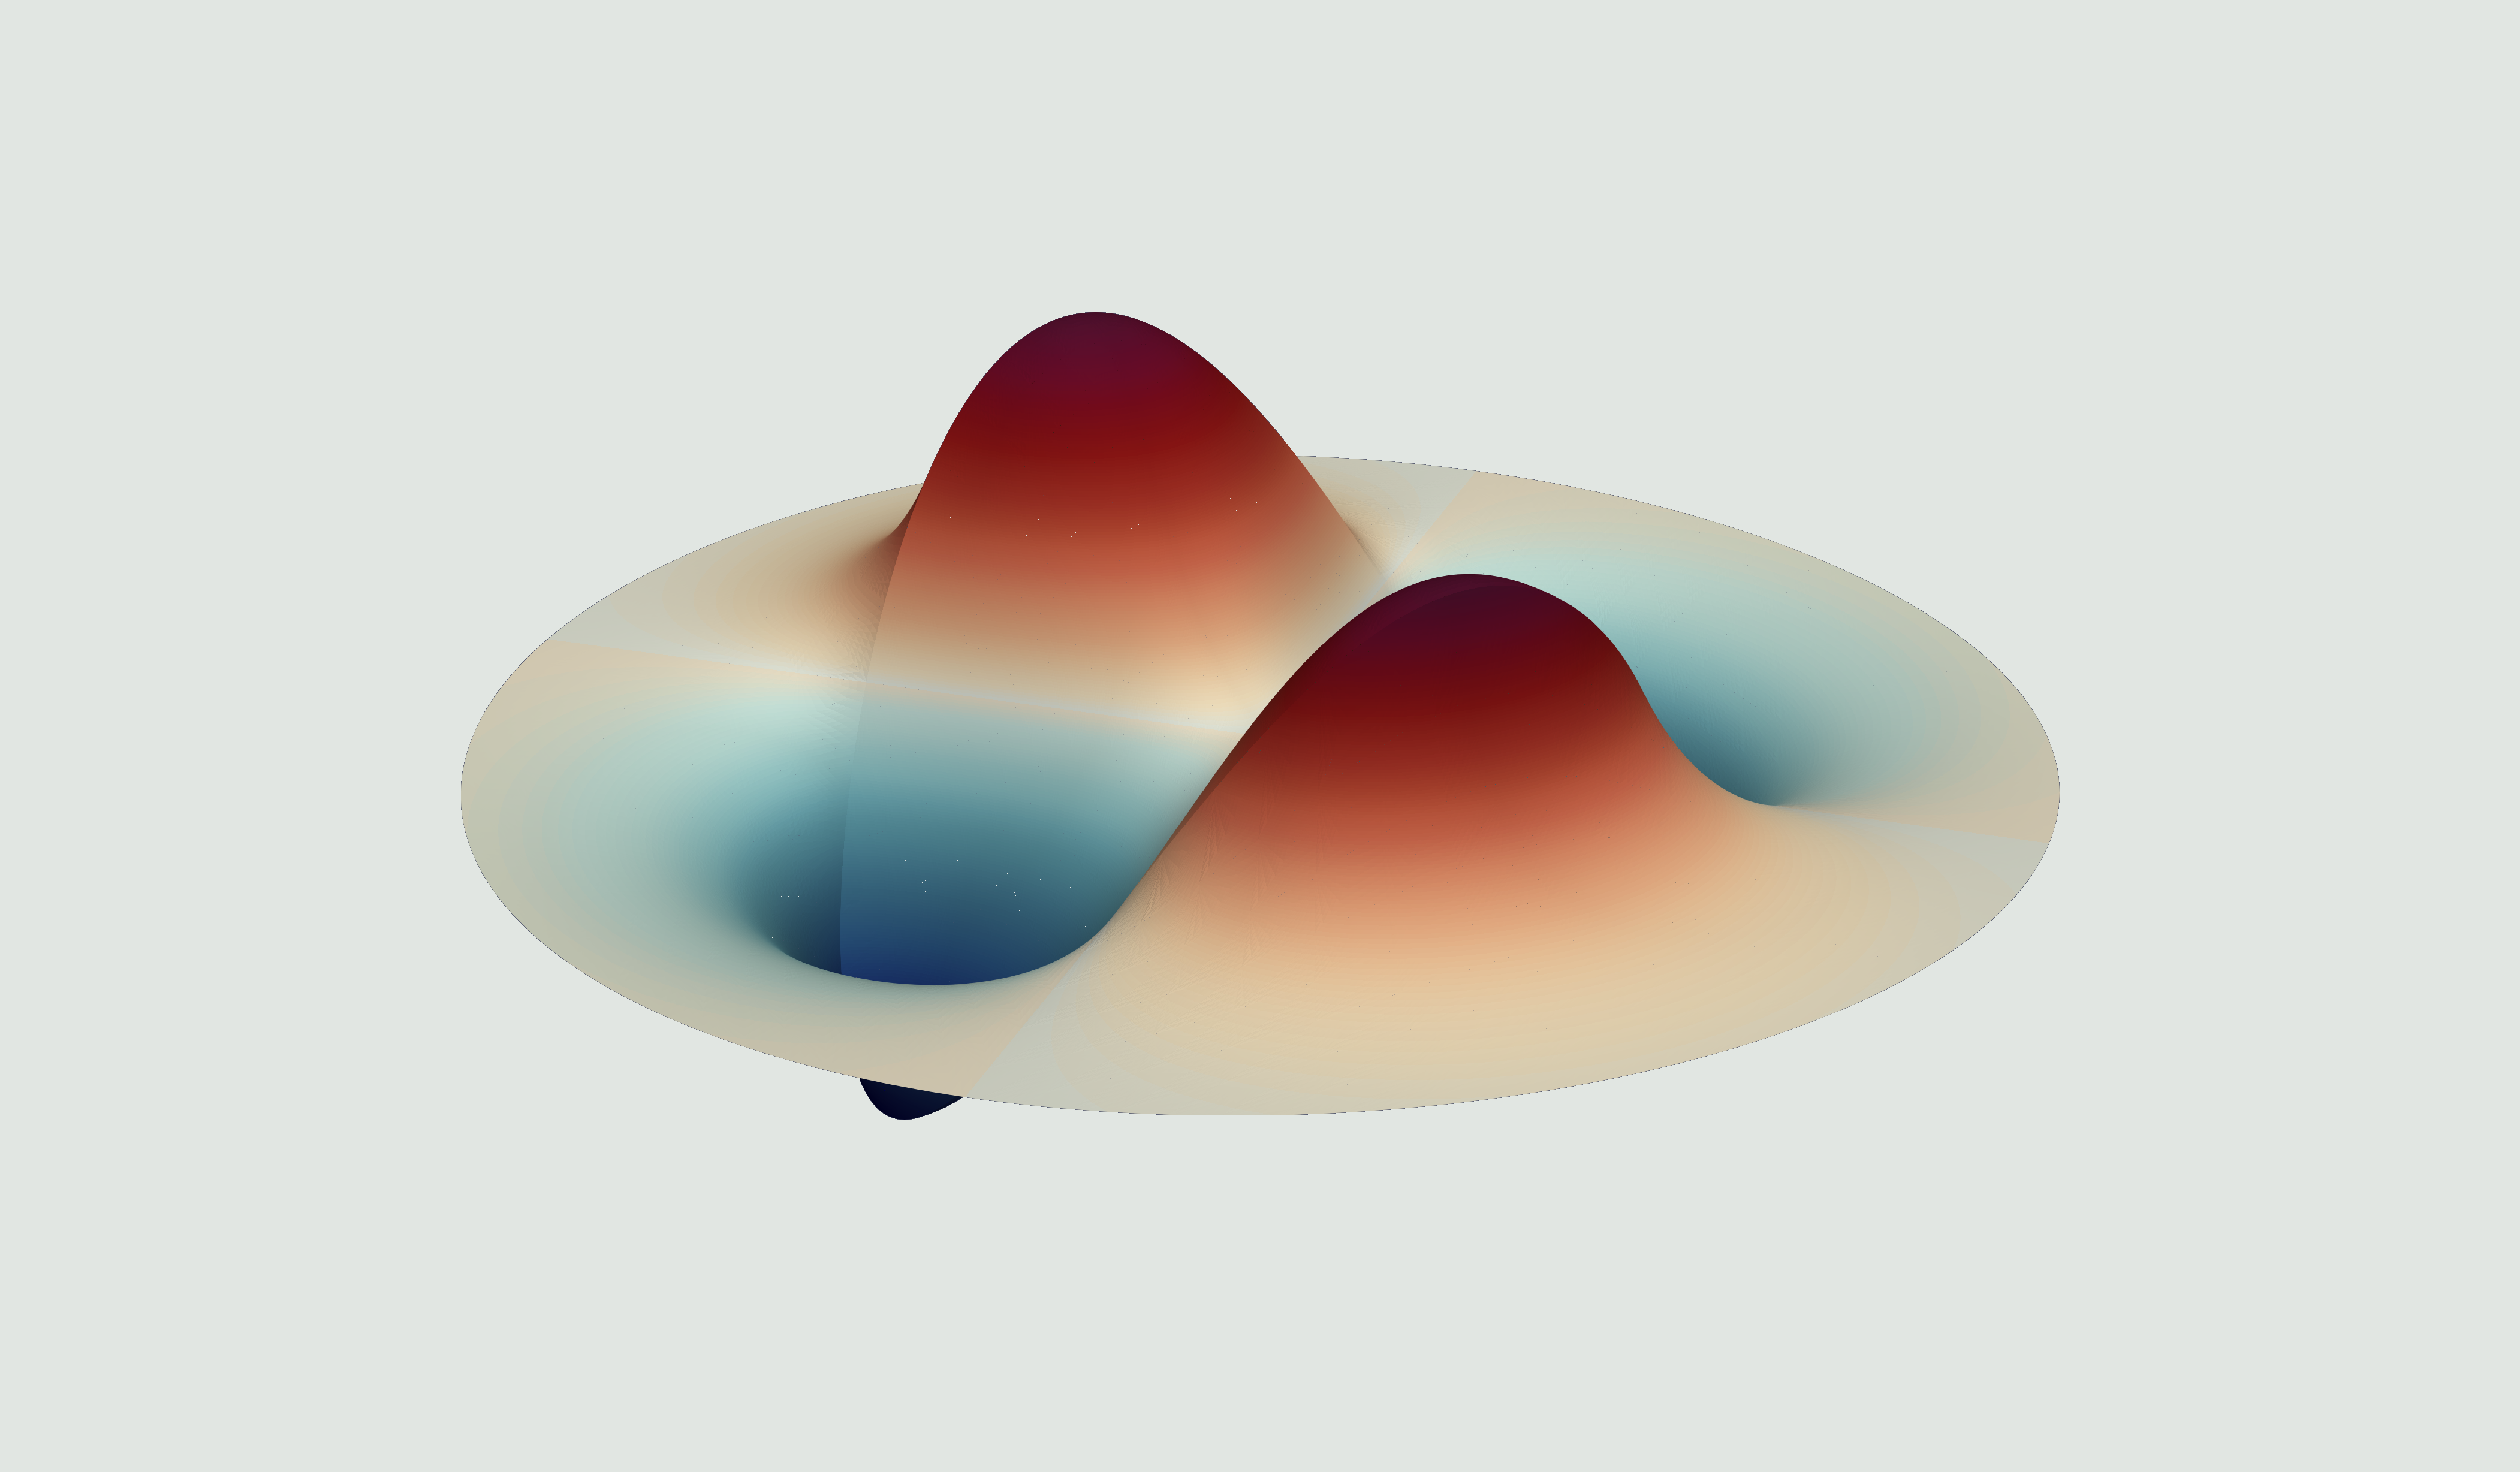
\includegraphics[width=1\linewidth]{images/ez3posterStepFiber.png}%
					\end{subfigure}
				\end{mdframed}
				\caption{These are really cool plots.}
				\label{fig:plot-step}
			\end{figure}
        \end{block}

        \vfill

      } % end of parbox
    \end{column}

    %% Right column:
    %% ============================================================
    \begin{column}{0.45\textwidth}
      \parbox[t][\columnheight]{\textwidth}{

        \vfill

        \begin{block}{\boxnumber HP-ADAPTIVITY CAPABILITIES }
        The developed basis functions, due to the hierarchical construction, can be integrated in the \emph{hp}-algorithms of the \texttt{NeoPZ} framework\parencite{diazcalle15}.

        \Cref{fig:mesh-holey} shows a \emph{hp}-adaptive mesh, in which the refinements were performed upon observation of the solution obtained with a fine mesh.
	        \begin{figure}
	        	\centering
		            \begin{tikzpicture}%
		        		\node[anchor=south west, inner sep=0] (X) at (0,0){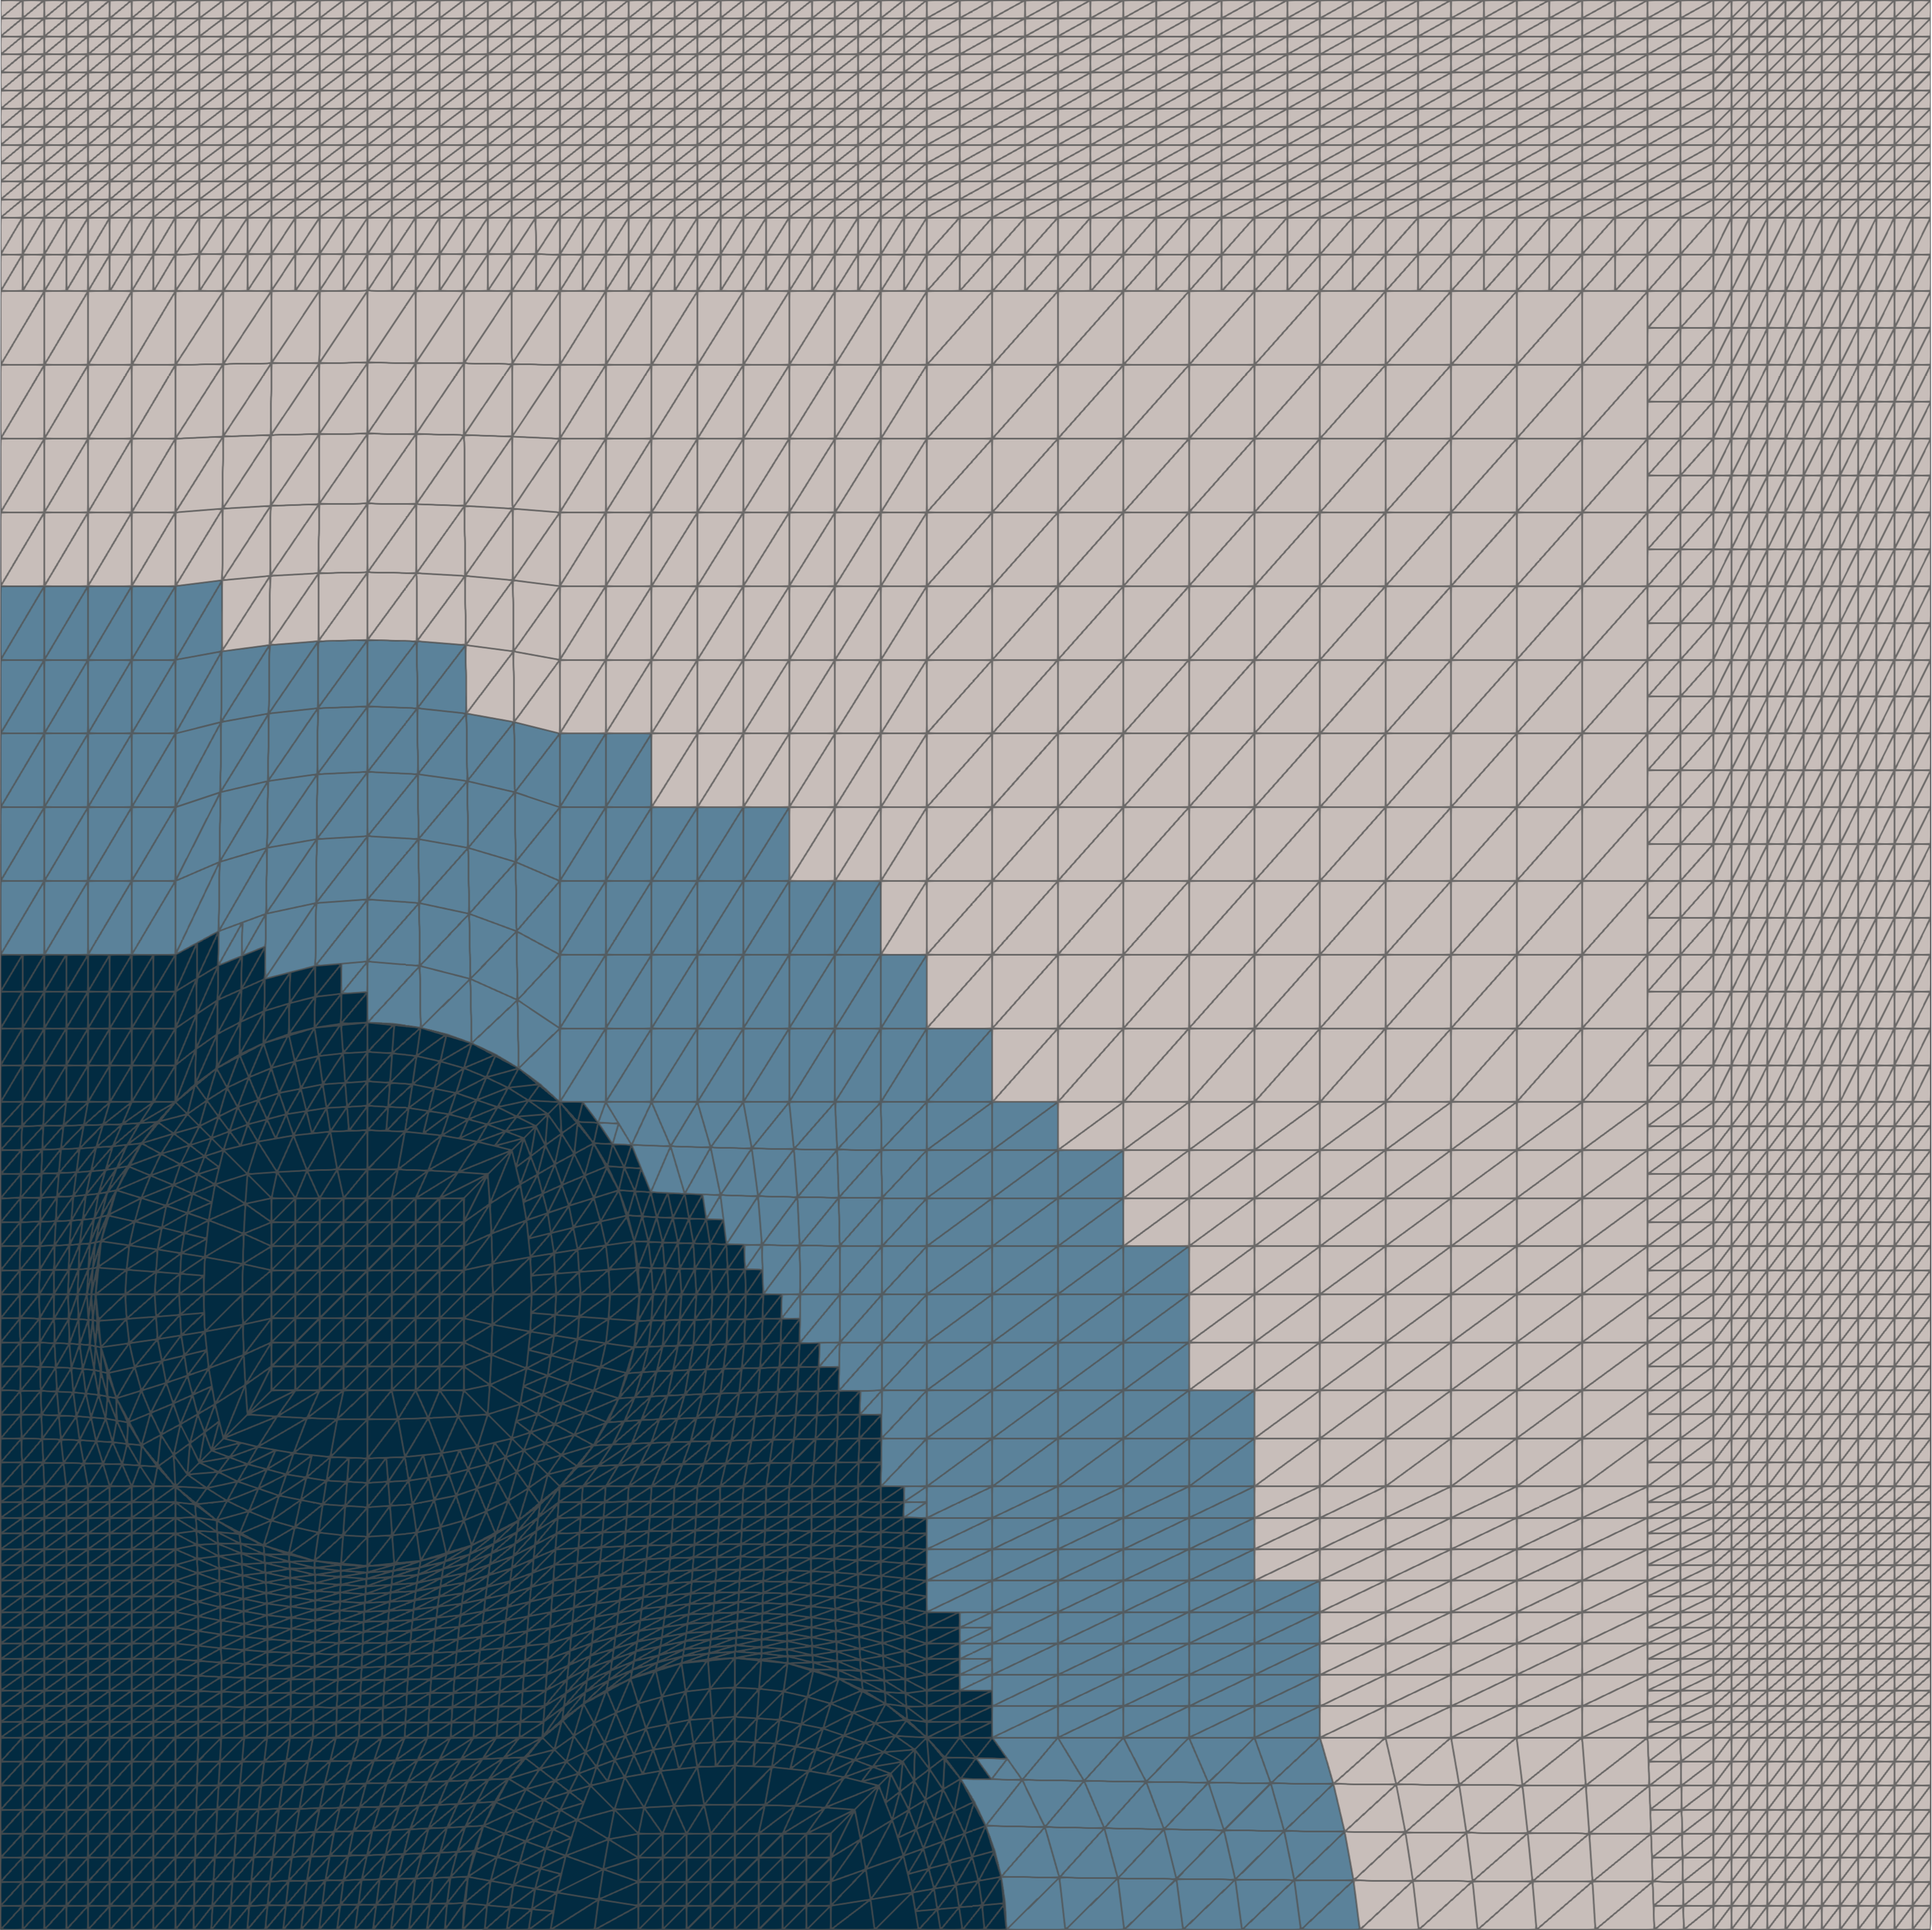
\includegraphics[height=0.8\linewidth]{images/holeyMesh.png}};%
		        		\begin{scope}[x={(X.south east)},y={(X.north west)}]%
		        		%% This makes all measurements with no units into fractions of the width
		        		%% and height of the graphic contained in the node.
		        		\draw[fill = white,fill opacity=0.8, text opacity=1] (0.05,0.075) rectangle (0.15,0.125) node[pos=.5] {$k=5$};
		        		\draw[fill = white,fill opacity=0.8, text opacity=1] (0.37,0.395) rectangle (0.47,0.445) node[pos=.5] {$k=4$};
		        		\draw[fill = white,fill opacity=0.8, text opacity=1] (0.65,0.675) rectangle (0.75,0.725) node[pos=.5] {$k=3$};
		        		\end{scope}%
		    	    \end{tikzpicture}
	    	    \caption{The Finite Element mesh of the microstructured fiber with six air-holes. The waveguide has a hole diameter of $d = 5\,\mu m$ and a hole pitch of $\Lambda=6.75\,\mu m$. The computational domain is a square with side $l=W+d_{pml}$, with $W=15.75\,\mu m$ and $d_{pml} = 2\, \mu m$. The elements have varying polynomial order from $k=3$ to $k=5$, and the mesh was refined on the region near the holes.}
	    	    \label{fig:mesh-holey}
	    	\end{figure}    	


			\begin{figure}[hb]
	        	\begin{mdframed}[backgroundcolor=bggrey]
					\centering
					\begin{subfigure}[b]{.4999\textwidth}
						\centering
						\caption*{$\displaystyle\bm{E}_t$}
						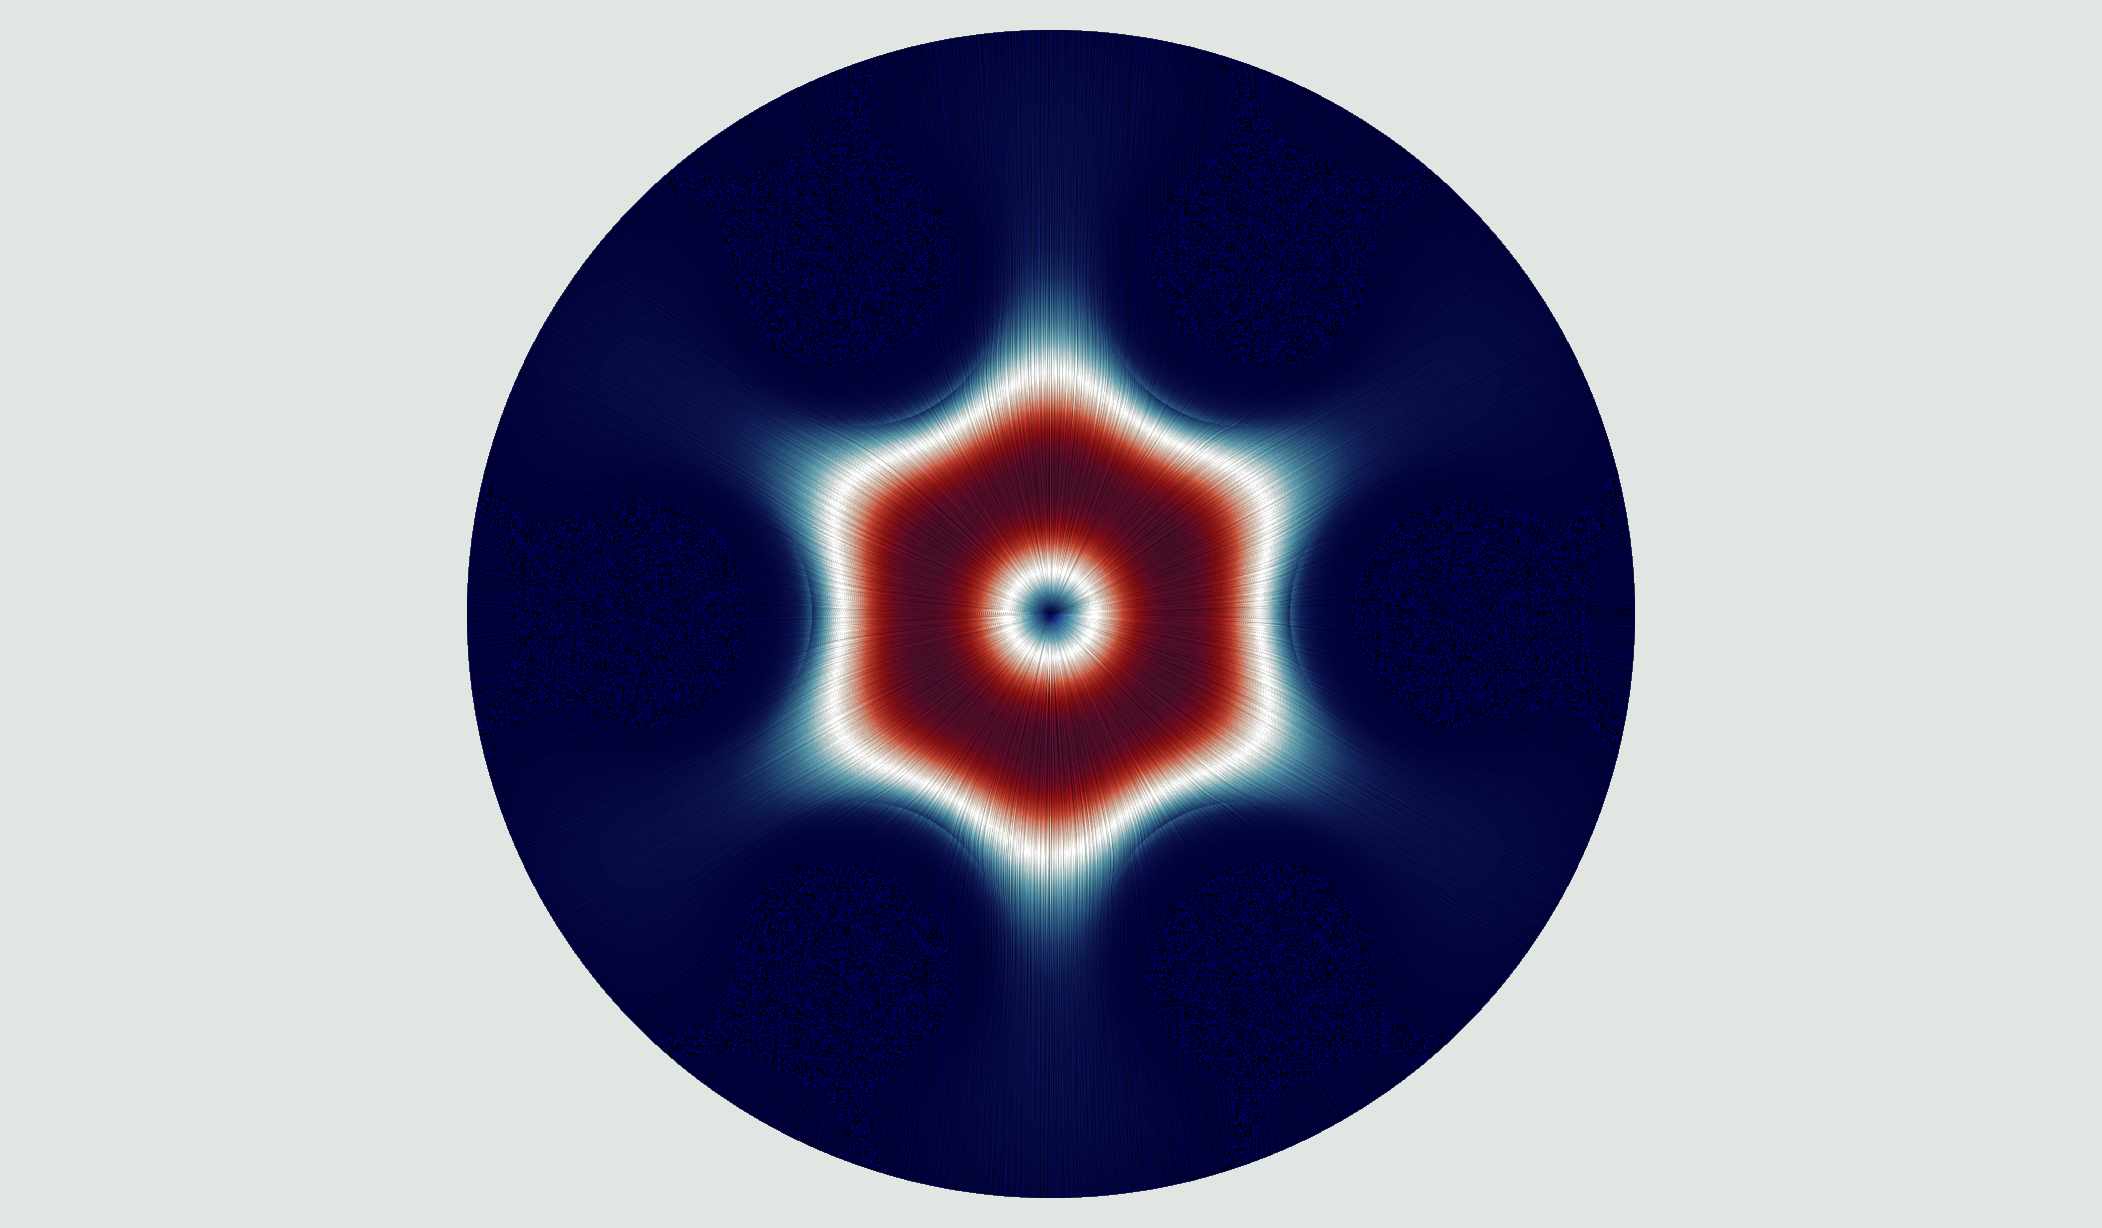
\includegraphics[width=1\linewidth]{images/et1posterHoley.png}%
					\end{subfigure}\hfill
					\begin{subfigure}[b]{.4999\textwidth}
						\centering
						\caption*{$\displaystyle E_z$}
						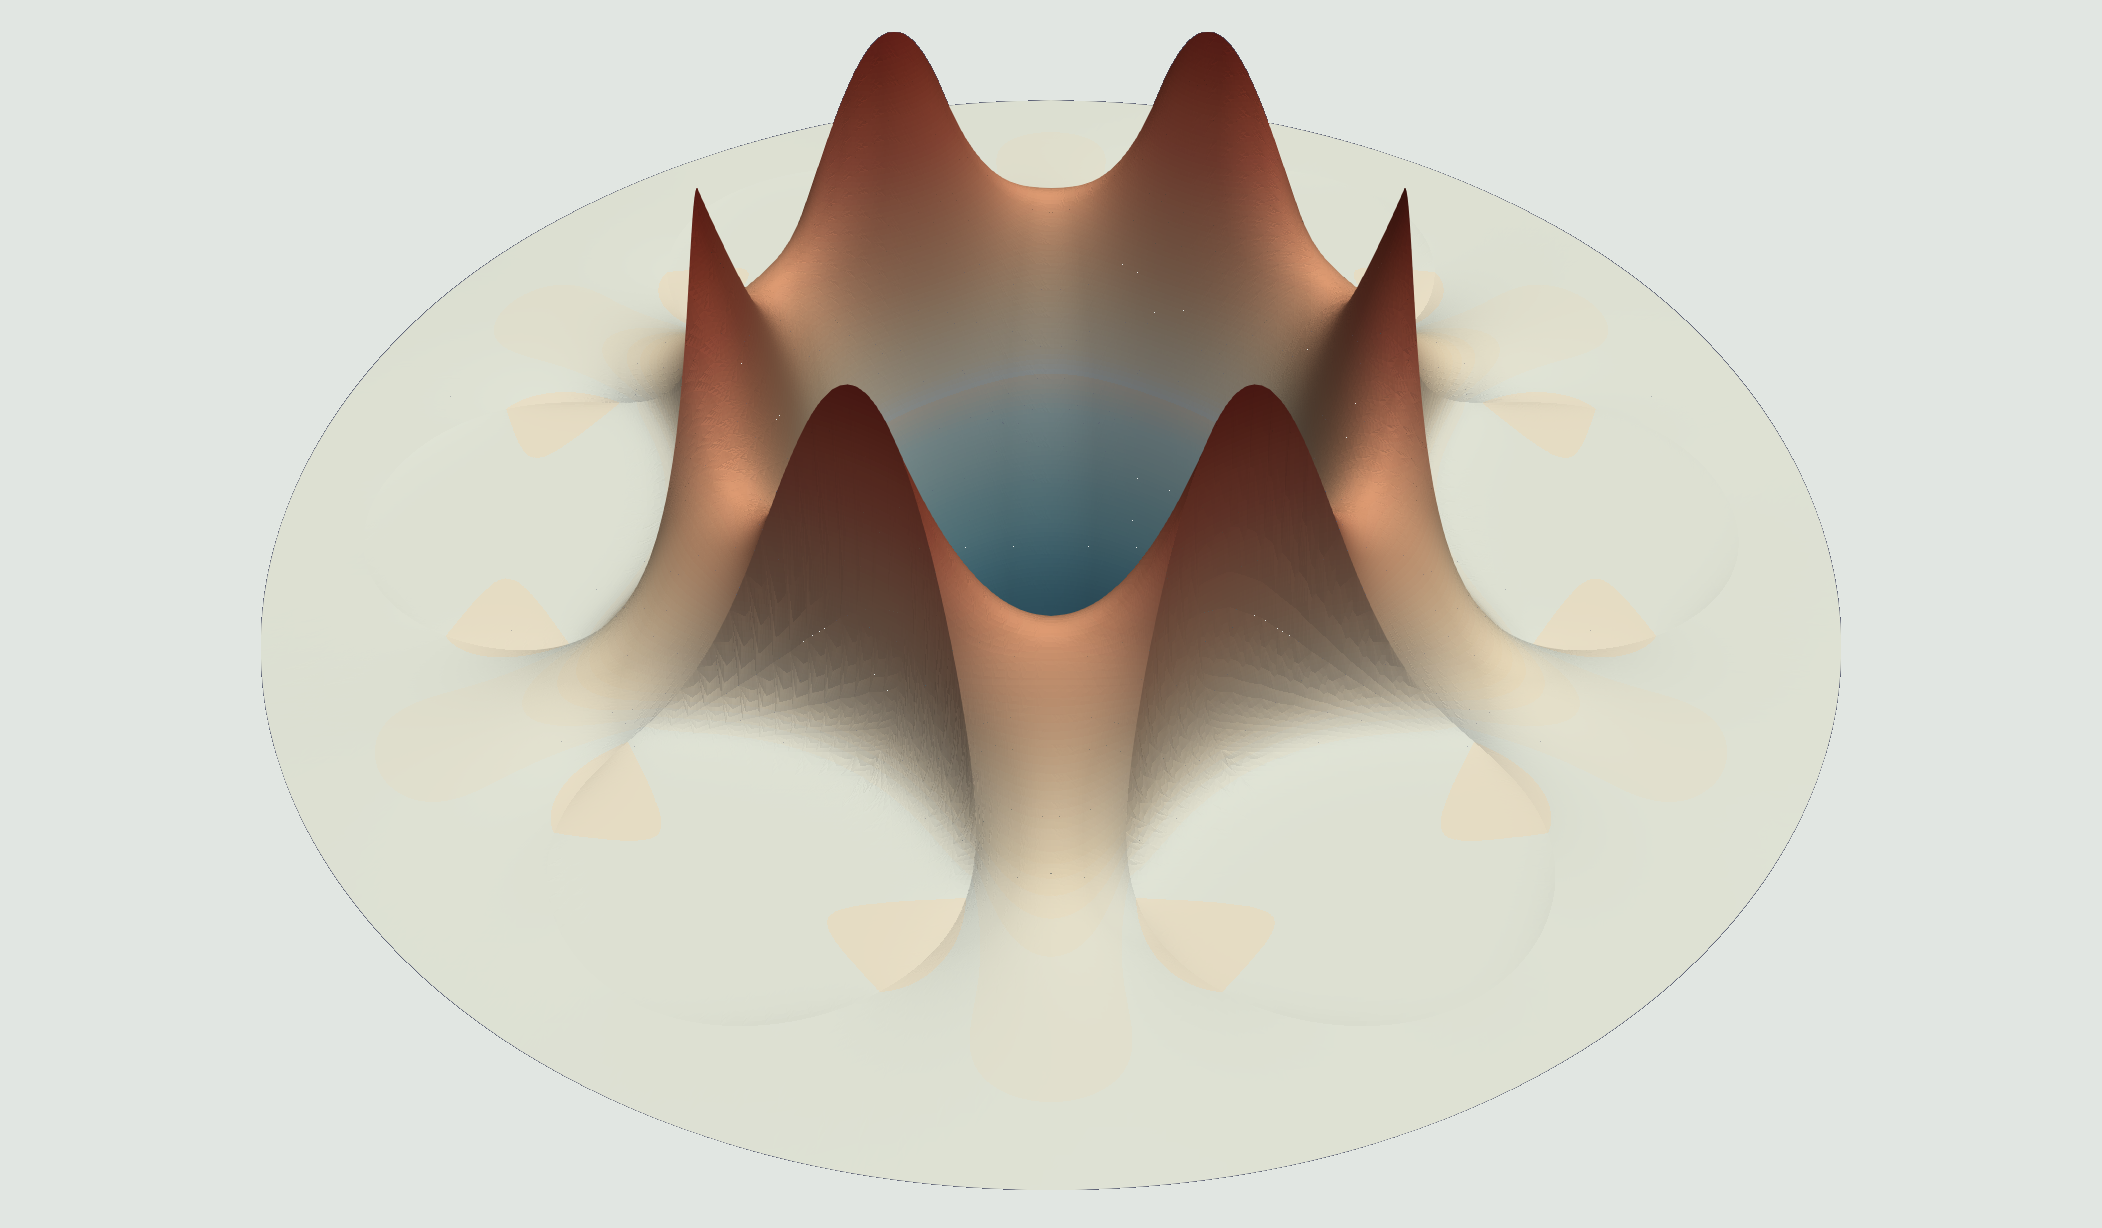
\includegraphics[width=1\linewidth]{images/ez1posterHoley.png}%
					\end{subfigure}

					\begin{subfigure}[b]{.4999\textwidth}
						\centering
						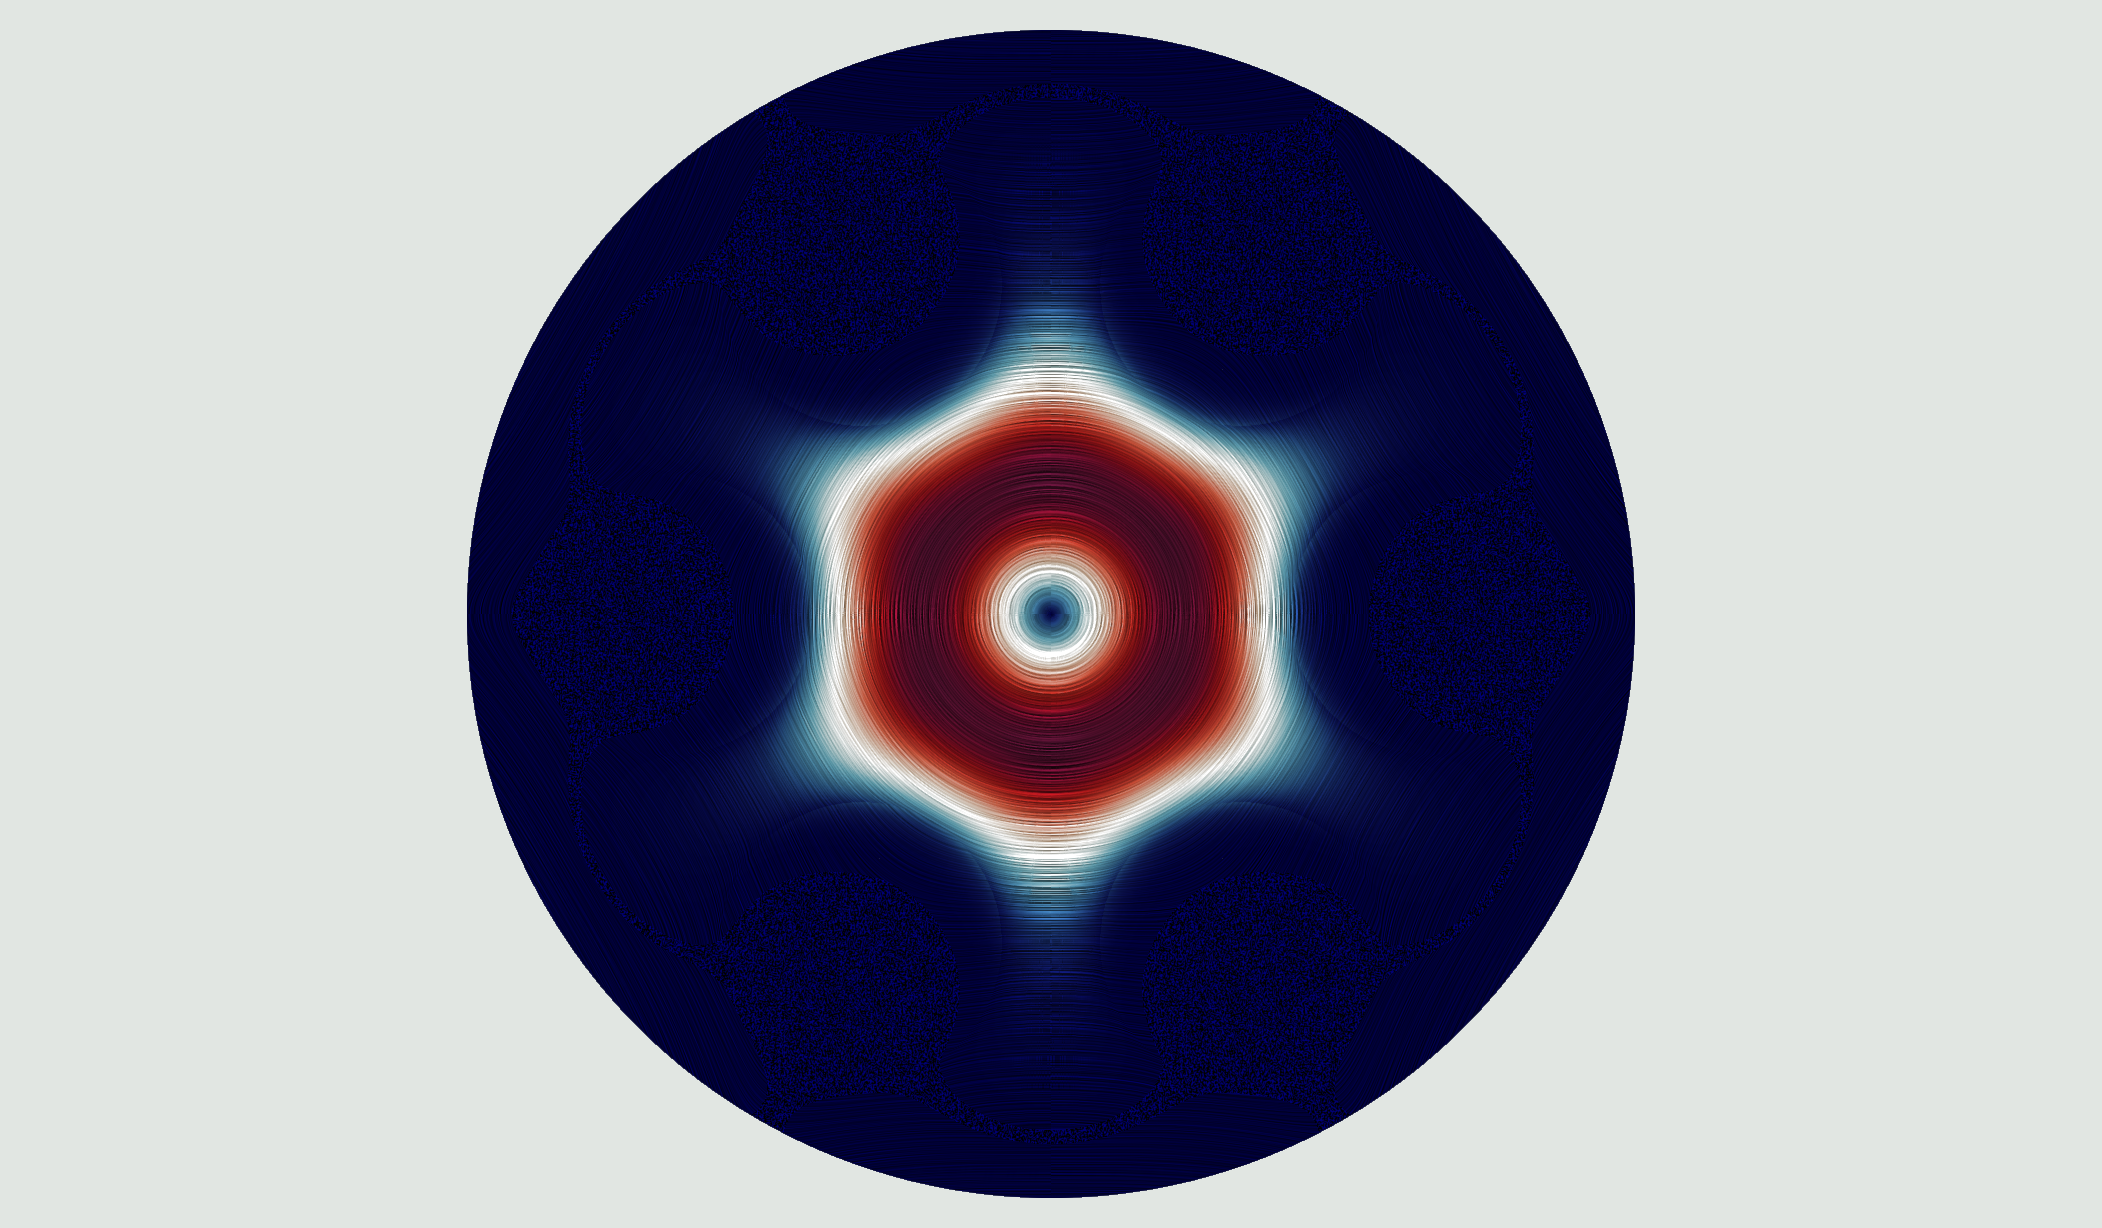
\includegraphics[width=1\linewidth]{images/et2posterHoley.png}%
					\end{subfigure}\hfill
					\begin{subfigure}[b]{.4999\textwidth}
						\centering
						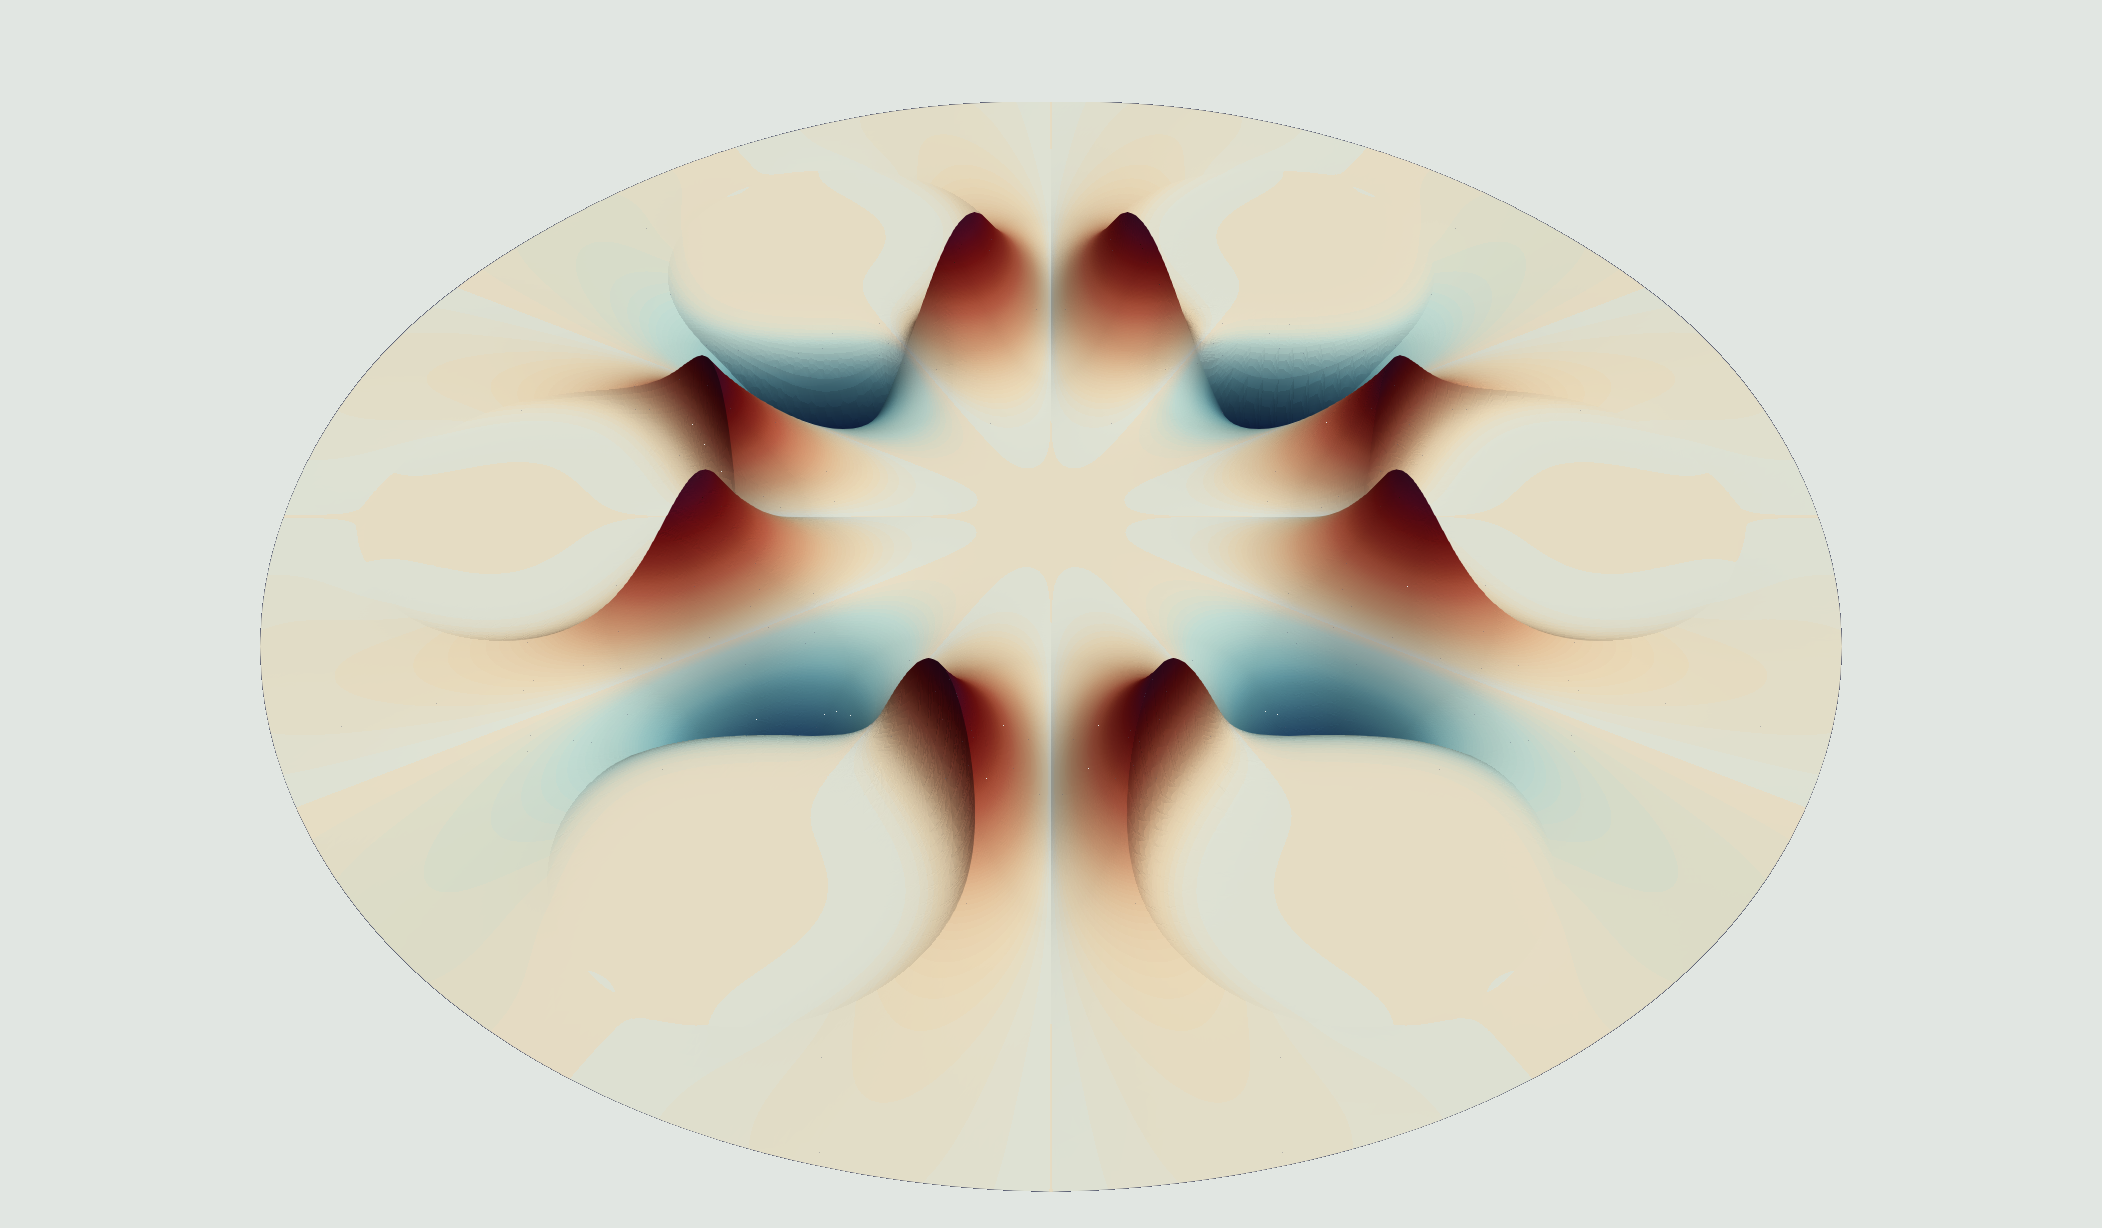
\includegraphics[width=1\linewidth]{images/ez2posterHoley.png}%
					\end{subfigure}
				\end{mdframed}
				\caption{These are also really cool plots.}
				\label{fig:plot-holey}
			\end{figure}
        \end{block}

        \vfill
        \begin{block}{REFERENCES}
        	\printbibliography
        \end{block}

        \vfill
      } % end of parbox
    \end{column}

  \end{columns}
\end{frame}

\end{document}
